% Options for packages loaded elsewhere
% Options for packages loaded elsewhere
\PassOptionsToPackage{unicode}{hyperref}
\PassOptionsToPackage{hyphens}{url}
\PassOptionsToPackage{dvipsnames,svgnames,x11names}{xcolor}
%
\documentclass[
]{article}
\usepackage{xcolor}
\usepackage[left=1in,right=1in,top=1in,bottom=1in]{geometry}
\usepackage{amsmath,amssymb}
\setcounter{secnumdepth}{-\maxdimen} % remove section numbering
\usepackage{iftex}
\ifPDFTeX
  \usepackage[T1]{fontenc}
  \usepackage[utf8]{inputenc}
  \usepackage{textcomp} % provide euro and other symbols
\else % if luatex or xetex
  \usepackage{unicode-math} % this also loads fontspec
  \defaultfontfeatures{Scale=MatchLowercase}
  \defaultfontfeatures[\rmfamily]{Ligatures=TeX,Scale=1}
\fi
\usepackage{lmodern}
\ifPDFTeX\else
  % xetex/luatex font selection
  \setmainfont[]{Latin Modern Roman}
\fi
% Use upquote if available, for straight quotes in verbatim environments
\IfFileExists{upquote.sty}{\usepackage{upquote}}{}
\IfFileExists{microtype.sty}{% use microtype if available
  \usepackage[]{microtype}
  \UseMicrotypeSet[protrusion]{basicmath} % disable protrusion for tt fonts
}{}
\makeatletter
\@ifundefined{KOMAClassName}{% if non-KOMA class
  \IfFileExists{parskip.sty}{%
    \usepackage{parskip}
  }{% else
    \setlength{\parindent}{0pt}
    \setlength{\parskip}{6pt plus 2pt minus 1pt}}
}{% if KOMA class
  \KOMAoptions{parskip=half}}
\makeatother
% Make \paragraph and \subparagraph free-standing
\makeatletter
\ifx\paragraph\undefined\else
  \let\oldparagraph\paragraph
  \renewcommand{\paragraph}{
    \@ifstar
      \xxxParagraphStar
      \xxxParagraphNoStar
  }
  \newcommand{\xxxParagraphStar}[1]{\oldparagraph*{#1}\mbox{}}
  \newcommand{\xxxParagraphNoStar}[1]{\oldparagraph{#1}\mbox{}}
\fi
\ifx\subparagraph\undefined\else
  \let\oldsubparagraph\subparagraph
  \renewcommand{\subparagraph}{
    \@ifstar
      \xxxSubParagraphStar
      \xxxSubParagraphNoStar
  }
  \newcommand{\xxxSubParagraphStar}[1]{\oldsubparagraph*{#1}\mbox{}}
  \newcommand{\xxxSubParagraphNoStar}[1]{\oldsubparagraph{#1}\mbox{}}
\fi
\makeatother

\usepackage{color}
\usepackage{fancyvrb}
\newcommand{\VerbBar}{|}
\newcommand{\VERB}{\Verb[commandchars=\\\{\}]}
\DefineVerbatimEnvironment{Highlighting}{Verbatim}{commandchars=\\\{\}}
% Add ',fontsize=\small' for more characters per line
\usepackage{framed}
\definecolor{shadecolor}{RGB}{241,243,245}
\newenvironment{Shaded}{\begin{snugshade}}{\end{snugshade}}
\newcommand{\AlertTok}[1]{\textcolor[rgb]{0.68,0.00,0.00}{#1}}
\newcommand{\AnnotationTok}[1]{\textcolor[rgb]{0.37,0.37,0.37}{#1}}
\newcommand{\AttributeTok}[1]{\textcolor[rgb]{0.40,0.45,0.13}{#1}}
\newcommand{\BaseNTok}[1]{\textcolor[rgb]{0.68,0.00,0.00}{#1}}
\newcommand{\BuiltInTok}[1]{\textcolor[rgb]{0.00,0.23,0.31}{#1}}
\newcommand{\CharTok}[1]{\textcolor[rgb]{0.13,0.47,0.30}{#1}}
\newcommand{\CommentTok}[1]{\textcolor[rgb]{0.37,0.37,0.37}{#1}}
\newcommand{\CommentVarTok}[1]{\textcolor[rgb]{0.37,0.37,0.37}{\textit{#1}}}
\newcommand{\ConstantTok}[1]{\textcolor[rgb]{0.56,0.35,0.01}{#1}}
\newcommand{\ControlFlowTok}[1]{\textcolor[rgb]{0.00,0.23,0.31}{\textbf{#1}}}
\newcommand{\DataTypeTok}[1]{\textcolor[rgb]{0.68,0.00,0.00}{#1}}
\newcommand{\DecValTok}[1]{\textcolor[rgb]{0.68,0.00,0.00}{#1}}
\newcommand{\DocumentationTok}[1]{\textcolor[rgb]{0.37,0.37,0.37}{\textit{#1}}}
\newcommand{\ErrorTok}[1]{\textcolor[rgb]{0.68,0.00,0.00}{#1}}
\newcommand{\ExtensionTok}[1]{\textcolor[rgb]{0.00,0.23,0.31}{#1}}
\newcommand{\FloatTok}[1]{\textcolor[rgb]{0.68,0.00,0.00}{#1}}
\newcommand{\FunctionTok}[1]{\textcolor[rgb]{0.28,0.35,0.67}{#1}}
\newcommand{\ImportTok}[1]{\textcolor[rgb]{0.00,0.46,0.62}{#1}}
\newcommand{\InformationTok}[1]{\textcolor[rgb]{0.37,0.37,0.37}{#1}}
\newcommand{\KeywordTok}[1]{\textcolor[rgb]{0.00,0.23,0.31}{\textbf{#1}}}
\newcommand{\NormalTok}[1]{\textcolor[rgb]{0.00,0.23,0.31}{#1}}
\newcommand{\OperatorTok}[1]{\textcolor[rgb]{0.37,0.37,0.37}{#1}}
\newcommand{\OtherTok}[1]{\textcolor[rgb]{0.00,0.23,0.31}{#1}}
\newcommand{\PreprocessorTok}[1]{\textcolor[rgb]{0.68,0.00,0.00}{#1}}
\newcommand{\RegionMarkerTok}[1]{\textcolor[rgb]{0.00,0.23,0.31}{#1}}
\newcommand{\SpecialCharTok}[1]{\textcolor[rgb]{0.37,0.37,0.37}{#1}}
\newcommand{\SpecialStringTok}[1]{\textcolor[rgb]{0.13,0.47,0.30}{#1}}
\newcommand{\StringTok}[1]{\textcolor[rgb]{0.13,0.47,0.30}{#1}}
\newcommand{\VariableTok}[1]{\textcolor[rgb]{0.07,0.07,0.07}{#1}}
\newcommand{\VerbatimStringTok}[1]{\textcolor[rgb]{0.13,0.47,0.30}{#1}}
\newcommand{\WarningTok}[1]{\textcolor[rgb]{0.37,0.37,0.37}{\textit{#1}}}

\usepackage{longtable,booktabs,array}
\newcounter{none} % for unnumbered tables
\usepackage{calc} % for calculating minipage widths
% Correct order of tables after \paragraph or \subparagraph
\usepackage{etoolbox}
\makeatletter
\patchcmd\longtable{\par}{\if@noskipsec\mbox{}\fi\par}{}{}
\makeatother
% Allow footnotes in longtable head/foot
\IfFileExists{footnotehyper.sty}{\usepackage{footnotehyper}}{\usepackage{footnote}}
\makesavenoteenv{longtable}
\usepackage{graphicx}
\makeatletter
\newsavebox\pandoc@box
\newcommand*\pandocbounded[1]{% scales image to fit in text height/width
  \sbox\pandoc@box{#1}%
  \Gscale@div\@tempa{\textheight}{\dimexpr\ht\pandoc@box+\dp\pandoc@box\relax}%
  \Gscale@div\@tempb{\linewidth}{\wd\pandoc@box}%
  \ifdim\@tempb\p@<\@tempa\p@\let\@tempa\@tempb\fi% select the smaller of both
  \ifdim\@tempa\p@<\p@\scalebox{\@tempa}{\usebox\pandoc@box}%
  \else\usebox{\pandoc@box}%
  \fi%
}
% Set default figure placement to htbp
\def\fps@figure{htbp}
\makeatother


% definitions for citeproc citations
\NewDocumentCommand\citeproctext{}{}
\NewDocumentCommand\citeproc{mm}{%
  \begingroup\def\citeproctext{#2}\cite{#1}\endgroup}
\makeatletter
 % allow citations to break across lines
 \let\@cite@ofmt\@firstofone
 % avoid brackets around text for \cite:
 \def\@biblabel#1{}
 \def\@cite#1#2{{#1\if@tempswa , #2\fi}}
\makeatother
\newlength{\cslhangindent}
\setlength{\cslhangindent}{1.5em}
\newlength{\csllabelwidth}
\setlength{\csllabelwidth}{3em}
\newenvironment{CSLReferences}[2] % #1 hanging-indent, #2 entry-spacing
 {\begin{list}{}{%
  \setlength{\itemindent}{0pt}
  \setlength{\leftmargin}{0pt}
  \setlength{\parsep}{0pt}
  % turn on hanging indent if param 1 is 1
  \ifodd #1
   \setlength{\leftmargin}{\cslhangindent}
   \setlength{\itemindent}{-1\cslhangindent}
  \fi
  % set entry spacing
  \setlength{\itemsep}{#2\baselineskip}}}
 {\end{list}}
\usepackage{calc}
\newcommand{\CSLBlock}[1]{\hfill\break\parbox[t]{\linewidth}{\strut\ignorespaces#1\strut}}
\newcommand{\CSLLeftMargin}[1]{\parbox[t]{\csllabelwidth}{\strut#1\strut}}
\newcommand{\CSLRightInline}[1]{\parbox[t]{\linewidth - \csllabelwidth}{\strut#1\strut}}
\newcommand{\CSLIndent}[1]{\hspace{\cslhangindent}#1}



\setlength{\emergencystretch}{3em} % prevent overfull lines

\providecommand{\tightlist}{%
  \setlength{\itemsep}{0pt}\setlength{\parskip}{0pt}}



 


\usepackage{booktabs}
\usepackage{longtable}
\usepackage{array}
\usepackage{multirow}
\usepackage{wrapfig}
\usepackage{float}
\usepackage{colortbl}
\usepackage{pdflscape}
\usepackage{tabularx}
\usepackage{xltabular}
\usepackage{threeparttable}
\usepackage{threeparttablex}
\usepackage[normalem]{ulem}
\usepackage{makecell}
\usepackage{xcolor}
\setlength{\footskip}{65pt}
\usepackage[font=scriptsize]{caption}
\usepackage[noblocks]{authblk}
\renewcommand*{\Authsep}{, }
\renewcommand*{\Authand}{, }
\renewcommand*{\Authands}{, }
\renewcommand\Affilfont{\small}
\renewcommand{\thefootnote}{\alph{footnote}}
\usepackage{etoolbox}
\AtEndEnvironment{abstract}{\noindent\textbf{Keywords:} \KeywordList \par}
\makeatletter
\@ifpackageloaded{caption}{}{\usepackage{caption}}
\AtBeginDocument{%
\ifdefined\contentsname
  \renewcommand*\contentsname{Table of contents}
\else
  \newcommand\contentsname{Table of contents}
\fi
\ifdefined\listfigurename
  \renewcommand*\listfigurename{List of Figures}
\else
  \newcommand\listfigurename{List of Figures}
\fi
\ifdefined\listtablename
  \renewcommand*\listtablename{List of Tables}
\else
  \newcommand\listtablename{List of Tables}
\fi
\ifdefined\figurename
  \renewcommand*\figurename{Figure}
\else
  \newcommand\figurename{Figure}
\fi
\ifdefined\tablename
  \renewcommand*\tablename{Table}
\else
  \newcommand\tablename{Table}
\fi
}
\@ifpackageloaded{float}{}{\usepackage{float}}
\floatstyle{ruled}
\@ifundefined{c@chapter}{\newfloat{codelisting}{h}{lop}}{\newfloat{codelisting}{h}{lop}[chapter]}
\floatname{codelisting}{Listing}
\newcommand*\listoflistings{\listof{codelisting}{List of Listings}}
\makeatother
\makeatletter
\makeatother
\makeatletter
\@ifpackageloaded{caption}{}{\usepackage{caption}}
\@ifpackageloaded{subcaption}{}{\usepackage{subcaption}}
\makeatother
\usepackage{bookmark}
\IfFileExists{xurl.sty}{\usepackage{xurl}}{} % add URL line breaks if available
\urlstyle{same}
\hypersetup{
  pdftitle={An updated systematic review and dose-response meta-analysis of protein intakes effects upon lean soft tissue mass{,} muscle{,} strength{,} and function in healthy adults},
  pdfauthor={James Steele; Everson Araujo Nunes; Myles Moore; Matthew Lees; Lauren Roxburgh; Andrea Viloria Medina; Stuart Phillips},
  pdfkeywords={protein, lean soft tissue mass, fat free
mass, muscle, strength, physical function, dose-response, resistance
training, bayesian},
  colorlinks=true,
  linkcolor={blue},
  filecolor={Maroon},
  citecolor={Blue},
  urlcolor={Blue},
  pdfcreator={LaTeX via pandoc}}


\title{An updated systematic review and dose-response meta-analysis of
protein intakes effects upon lean soft tissue mass, muscle, strength,
and function in healthy adults\thanks{Preprint, please cite as: Steele,
J., Nunes, E.A., Moore, M., Lees, M., Roxburgh, L., Viloria Medina, A.,
and Phillips, S. (2026). An updated systematic review and dose-response
meta-analysis of protein intakes effects upon lean soft tissue mass,
muscle, strength, and function in healthy adults. sportrxiv DOI:
\url{https://doi.org/10.51224/SportRxiv.????}. Address for
correspondence: james@steele-research.com}}


\author[1,2,3]{James Steele}
\author[4]{Everson Araujo Nunes}
\author[5,6]{Myles Moore}
\author[7]{Matthew Lees}
\author[7]{Lauren Roxburgh}
\author[7]{Andrea Viloria Medina}
\author[7]{Stuart Phillips}

\affil[1]{Steele Research Limited, Eastleigh, Hampshire, UK}
\affil[2]{MacroFactor, Stronger by Science Technologies LLC, Raleigh,
North Carolina, USA}
\affil[3]{School of Health and Biomedical Sciences, Royal Melbourne
Institute of Technology, Melbourne, VIC, Australia}
\affil[4]{College of Biological Science, Department of Human Health
Sciences, University of Guelph, Guelph, Ontario, Canada}
\affil[5]{Kieser Australia, Melbourne, VIC, Australia}
\affil[6]{Tasmanian Centre for Mental Health Service Innovation,
Tasmanian Health Services, Hobart, TAS, Australia}
\affil[7]{Department of Kinesiology, McMaster University, Hamilton,
Ontario}

% Store the keywords (expanded by Pandoc here)
\def\KeywordList{protein, lean soft tissue mass, fat free
mass, muscle, strength, physical function, dose-response, resistance
training, bayesian}

\date{July 26, 2026}
\begin{document}
\maketitle
\begin{abstract}
TO WRITE
\end{abstract}


\section{Introduction}\label{introduction}

In a recent systematic review and meta-analysis Nunes et al. (2022)
examined the dose-response effects of protein intake relative to body
mass upon lean soft tissue mass, muscle mass/size, strength, and
function both with and without concomittant resistance training (RT).
However, whilst they examined both categorical protein intakes
(`\textless1.2 g/kg/day', `1.2--1.59 g/kg/day' and `≥1.6 g/kg/day') as
well as continuous (as g/kg/day) in the the latter only linear
functional forms were utilised which imply a constant slope of proteins
effect across varied intakes. It may be the case that some kind of
non-linear functional form may better describe the dose-response
relationship. For example, in earlier work Morton et al. (2018) used a
piecewise linear model and estimated a so-called ``breakpoint'' where a
plateau in protein intakes effects might occur for lean soft tissue
(breakpoint = 1.62 g/lg/day {[}95\%CI: 1.03, 2.20{]}) . Tagawa et al.
(2021; 2022) have also reported possible non-linear functional forms
where they utilised piecewise splines though inflexion points were
selected arbitrarily; 1.3 g/kg/day for strength outcomes without RT and
for lean soft tissue mass with RT, and 1.5 g/kg/day for strength
outcomes with RT). However, both approaches are somewhat limited in
specifically forcing a single ``breakpoint''. Instead, more flexible
modelling strategies using extensions of generalised additive models to
meta-analytic scenarios may allow for clearer determination of the
dose-response function based on existing studies data. Further, the use
of singular models renders dose-response estimates conditional on that
particular model (e.g., a linear model can only produce a linear dose
response function, or the inclusion of a singular breakpoint will only
allow the model to ``flex'' about that point).

Whilst the models previously explored may have plausibility, at least
over the range of data available, these previous analyses have also not
made any attempts at comparing functional forms implied by different
models. However, even comparing amongst different candidate models with
regards to the relative evidence for and against different functional
forms as being the underlying data generating process has limitations.
Any predictions are conditional on the candidate model selected and
selection process. Indeed, when fitting models to data, even when all
are plausible candidates, there is uncertainty in the possible models
that could be fit and the selection process. However, with Bayesian
approaches to modelling it is simple to combine, in a weighted fashion
determined by their relative evidence, estimates from all models
examined and directly incorporate this uncertainty ({Hinne et al.},
2020). Adopting a Bayesian approach for evidence synthesis also allows
the incorporation of prior information that might be relevant to
inference. For example, we also have precise estimates of the effects of
RT without additional protein intervention from previous meta-analyses
for lean soft tissue mass, muscle mass/size, strength, and functional
outcomes (Kirk et al., 2024; Steele et al., 2023). Most, though not all,
previous protein intake intervention studies have examined RT as a
concomitant intervention. As such we can also utilise these estimates,
in addition to those from non-RT control groups, to set informative
priors for the expected effect sizes at habitual protein intakes (i.e.,
the typical protein intakes of people taking part in intervention
research examining RT without a concomitant intervention to increase
protein intake).

Previous meta-analyses examining the effects of protein intake upon the
outcomes noted have typically not pre-registered a smallest effect size
of interest range to draw conclusions regarding the meaningfulness of
the effects identified. Here we also set the smallest effect size of
interest to interpret the how meaningful the effects of increased
protein intake are upon outcomes. This would enable both current
recommendations to be updated if necessary and also generate a
functional form enabling more precise theoretical predictions of effects
that future studies might offer severe tests of i.e., predicted
magnitudes of condition by time interaction effects for comparing
different doses of protein in a randomised trial.

Thus, we sought to revisit the studies that were included in the review
of Nunes et al. (2022), in addition to updating searches since the date
of their last search to include any newer studies replicating and
extending the systematic searches conducted previously. Our aim was to
explore the dose-response relationships between experimental
manipulation of protein intake and both lean soft tissue mass, muscle,
strength, and function in healthy adults.

\section{Methods}\label{methods}

This systematic review was originally pre-registered in July 2025 on the
Open Science Framework following the structure for registration with the
International Prospective Register of Systematic Reviews (PROSPERO). The
pre-registration and any updates to it is available at:
\url{https://osf.io/w2qpx/overview}. We followed the Preferred Reporting
Items for Systematic Reviews and Meta-Analyses (PRISMA) guidelines (Page
et al., 2021).

\subsection{Updates to
pre-registration}\label{updates-to-pre-registration}

Some minor ammendments were made to our analysis plan after
pre-registeration when we realised that protein intake as a predictor
for the arm level within studies is also estimated with error (i.e.,
sampling error) where it is a combination of dietary intake
(experimentally manipulated or not) and any experimentally manipulated
supplementation to increase protein intake. As such, we updated our
approach and extracted sufficient data from all included studies to
enable us to either use the reported standard errors for protein intake
in g/kg/day, or to propagate error in the calculation of protein intake,
and to then model this directly using latent error models for the
predictor. In addition a typo in the priors was noted where the scale
for weakly regularising priors on coefficients other than the effects of
RT was set to 10 when it should have been 1 given the former allows for
completely implausible standardised mean changes Lastly, instead of the
slopes at different protein intakes for the magnitude of the median
difference between intervention and control arms, we have updated to
consider the paired contrasts across the dose-response function for
different protein intakes in contrast with the recommended daily
allowance of 0.8 g/kg/day as the reference condition.

\subsection{Search Strategy}\label{search-strategy}

The search strategy used by Nunes et al. (2022) as replicated exactly
with searches and screening being conducted by two investigators (EAN,
ML) with any disagreements planned to be resolved by a third
investigator (JS) though no disagreements occured. The original search
strategy can be seen in the online supplementary materials for Nunes et
al. (2022)
\href{https://onlinelibrary.wiley.com/action/downloadSupplement?doi=10.1002\%2Fjcsm.12922&file=jcsm12922-sup-0005-Search_strategies_.pdf}{here}.
Searches had previously been conducted up to September 2020 by Nunes et
al. (2022) and so we performed searches from this date up to July 2025.
In addition, any papers not identified in the original or updated
searches but which were known to the author team and met inclusion
criteria were also identified and included. Rayyan (Ouzzani et al.,
2016) was used to manage the screening process after searches were
conducted.

\subsection{Inclusion/exclusion
criteria}\label{inclusionexclusion-criteria}

We will examined studies including healthy adults and which manipulated
protein intake experimentally with or without inclusion of a concomitant
RT intervention performed in any settings. The following population,
intervention, comparator, and outcomes (PICO) was used to guide
inclusion:

\begin{itemize}
\tightlist
\item
  Population

  \begin{itemize}
  \tightlist
  \item
    Adult participants (healthy) aged 18 years or older.
  \end{itemize}
\item
  Intervention(s) or exposure(s)

  \begin{itemize}
  \tightlist
  \item
    Additional protein ingestion with or without the addition of
    resistance exercise (increasing protein ingestion as the primary
    intervention using nutritional supplements or diet at any dose or
    level).
  \end{itemize}
\item
  Comparator(s) or control(s)

  \begin{itemize}
  \tightlist
  \item
    Placebo or no intervention (control).
  \end{itemize}
\item
  Outcomes

  \begin{itemize}
  \tightlist
  \item
    Lean soft tissue mass (or a closely related measure i.e., fat-free
    mass; Heymsfield et al. (2024)), direct measures of muscle mass/size
    (both whole muscle and muscle fiber), muscle strength and
    performance in tests of physical function.
  \end{itemize}
\end{itemize}

Studies including participants with decreased mobility, frailty,
obesity, or any chronic or infectious diseases were not included. Also,
interventions were carefully screened for the presence of any potential
active ingredient that might impact lean soft tissue mass gain other
than protein (i.e.~creatine, phosphatidic acid, omega-3 fatty acids,
anabolic steroids, and beta-hydroxy-beta-methylbutyrate {[}HMB{]}) or if
they were intended to cause weight loss (e.g., energy restriction). If a
particular study testing potential active supplements had intervention
groups fitting our inclusion criteria, the study was included and
assessed to extract the respective arm based data of protein and
control/placebo interventions only. No restrictions were imposed
regarding additional protein dose or the duration of the intervention
protocol. Only randomised controlled trials using parallel arm designs
(i.e., where arms where independent) were included.

For primary outcomes we considered the following as valid
operationalisations of these constructs: for whole body lean soft tissue
mass, dual-energy X-ray absorptiometry (DEXA), hydrodensitometry,
bioimpedance analysis (BIA), skinfolds, and/or whole-body air
plethysmography (BodPod®); for direct measures for muscle size/mass,
magnetic resonance imaging (MRI), computed tomography (CT), ultrasound
(US), appendicular measures of muscle mass using DEXA or BIA, and any
muscle biopsy measures for fiber cross sectional area; for strength, any
repetition-maximum (isotonic), maximal isometric, or maximal isokinetic
testing for all tasks/exercises; and for physical function, timed up and
go (TUG), chair-based testing (i.e., sit to stand), sit-to-stand tests,
gait speed tests, balance tests, short physical performance battery
tests, stair climb tests, time or distance-limited walking tests, jump
tests, agility tests, flexibility tests, and any other tests involving
activities of daily life.

\subsection{Data extraction/coding}\label{data-extractioncoding}

It was originally planned that data would be extracted by at least two
investigators after random allocation of newly identified studies with
discrepancies checked by a third (JS). However, two members of the
original extraction team were unable to complete their extraction and so
two authors (LR, AVM) extracted the studies allocated to them with a
third (JS) going back through all included studies, including
re-extracting data from the original studies included in Nunes et al.
(2022) in addition to all newly identified studies, such that all
studies had been checked and extracted by at least two authors.

For each study we extractedd bibliometric data including pubmed ID, DOI,
authors, corresponding author email, journal, year of publication, title
of article, and how many arms from the study were to be included in our
analysis. For each arm within each study data was extracted participant
characteristics, including location (i.e., means) and scale (i.e.,
standard error, or standard deviations) for any continuous variables,
which included sex (proportion male), age and body mass, sample size at
baseline, intervention characteristics including protein source and what
the placebo arm consisted of, whether concomitant RT was performed, and
dietary protein intake (at baseline and during the study i.e., after
intervention). On an arm by arm basis, and for each time point reported
in the study, all whole body lean soft tissue mass and direct muscle
mass/size outcomes, strength outcomes, and function outcomes in addition
to the outcome group they belong to (whole body lean soft tissue mass;
direct muscle size/mass; strength; function), the measurement method,
the units of measurement, samples sizes, and means and either standard
deviations, standard errors, or confidence intervals were extracted in
addition to contrasts between each time points mean deltas (e.g., for
two timepoints 1 and 2, timepoint 2 -- timepoint 1) and their standard
deviations or standard errors, t statistics, p values, confidence
intervals, and correlation between timepoints. If not available in
tables or the text, data was extracted from figures using the online
tool WebPlotDigitizer (all data extracted from figures is available in
the online supplementary materials). Authors were contacted for missing
data. We originally planned to contact all authors to request individual
participant level data, however utlimately opted not to pursue this due
to resource and time constraints for the author team to commit to this.

\subsection{Risk of bias and quality of evidence
assessment}\label{risk-of-bias-and-quality-of-evidence-assessment}

The RoB2 tool (Sterne et al., 2019) was used to examine risk of bias in
the included studies, both those included in Nunes et al. (2022) and all
newly identified studies. Further the quality of evidence was appraised
using the GRADE criteria.

\subsection{Statistical analysis}\label{statistical-analysis}

Statistical analysis of the data extracted was be performed in R (v
4.4.3; R Core Team, https://www.r-project.org/) and RStudio (v
2026.07.0; Posit, https://posit.co/). All of the code utilized for the
data preparation and analyses is available on the Open Science Framework
page (\url{https://osf.io/37bzv/} and the corresponding GitHub
repository
(\url{https://github.com/jamessteeleii/protein_dose_response_meta}).

\begin{verbatim}
We cite all software and packages used in the analysis pipeline using the `grateful` package [@rodriguez-sanchezGratefulFacilitateCitation2023] which can be seen here: [https://jamessteeleii.github.io/project_DS_volume/grateful-report.html](https://jamessteeleii.github.io/project_DS_volume/grateful-report.html).
\end{verbatim}

Standardised mean changes with small sample bias correction were
calculated within each arm and for each outcome for each contrast
relative to baseline using Becker's (1988) \(d\) (i.e., where the
numerator is the mean for a given follow-up timepoint, n, after baseline
minus the mean for baseline; timepoint 0+n - timepoint 0; where only
mean delta contrasts between timepoints are reported, though baseline
standard deviations are available, we used the delta score for the
contrast to baseline as the numerator). However, given we are including
only randomised controlled trials we will use the pooled baseline
standard deviations as the denominator, akin to Morris' (2008)
\(PPC_2\), given that participants come from the same population at
randomisation. We used standardised mean change scores due to the
varying outcome operationalisations for the constructs considered (i.e.,
in both specific method of observation and in the units of measurement)
that were extracted. Further, given the nature of the constructs of
interest this facilitated comparison with other large scale
meta-analytic estimates (e.g., Steele et al. (2023)) to enable
interpretation of the magnitude of effects identified.

Though we have specific criteria for the selected models described below
that were fit, our analysis should be considered exploratory and aimed
at principled dose-response model selection. Our dependent variable in
all models is the standardised mean change relative to baseline at each
follow-up timepoint calculated as described above. Analysis was aimed at
effect estimation within a Bayesian meta-analytic framework (Kruschke \&
Liddell, 2018). For all analyses, the model estimates and their
precision, along with conclusions based upon them, are interpreted
continuously and probabilistically, considering the data quality, the
plausibility of effect, and the previous literature, all within the
context of our models.

We originally planned to use the main package \texttt{brms} (Burkner,
2018) in fitting all the Bayesian meta-analysis models described below.
We still report the results of these models as our primary analysis.
However, as noted above we subsequently realised that our primary
predictor of protein intake is one estimated with error (i.e., sampling
error) for each study and arm included. As such, we updated our approach
and extracted sufficient data from all included studies to enable us to
either use the reported standard errors, or to propagate error in the
calculation of protein intake, and to then model this directly using
measurement error models for the predictor. Therefore, all models remain
the same, or as closely as possible, in terms of their described
function forms if not exactly in their parameterisation, for fitting and
inclusion of covariates and random effects, but instead the
\texttt{brms} models were translated to Stan models in order to fit them
using \texttt{cmdstanr} with this latent error in variables approach.
Essentially this treated each estimate of protein intake as an estimate
with error and for which the underlying true protein intake was modelled
as a latent parameter and it was this which was treated as the predictor
within each higher model. These errors in variables models are reported
in the supplementary materials. We used four Monte Carlo Markov Chains
each with 2000 warmup and 6000 sampling iterations. Note this deviated
from our pre-registration in order to reduce the time required for model
fitting given that we were primarily interested in estimation rather
hypothesis testing and so did not calculate Bayes Factors. Trace plots
were produced along with rhat values to examine whether chains were
converged for each model, and posterior predictive checks for each model
were also examined to understand the model implied distributions. These
were examined across all models prior to comparisons to ensure good
convergence, that all rhat values were close to 1, and posterior
predictive checks seem appropriate distributions for the observed data.
Prior and posterior draws for both global grand means of marginal
predictions and marginal contrasts for protein intakes at intervals of
0.2 g/kg/day with 0.8 g/kg/day set as the reference intake and contrasts
with this up to 4.4 g/kg/day (i.e., the highest protein intake point
estimate reported in the included studies).

Data was hierarchical across three levels (i.e., effects within arms
within studies), and so, we included random (i.e., cluster) intercepts
using implicit nested coding across these levels in all models. We then
examined a selection of models for the functional form of dose-response
effect of protein intake. For each model, protein intake was included as
a fixed (i.e., population) effect in g/kg/day and centred at the median
value for protein intake across all control and placebo arms i.e.,
considered to be the habitual protein intake, which was 1.1 g/kg/day. In
all models we included a dummy coded fixed effect for whether the study
included a RT intervention (code = 0) or not (code = 1) and set
informative priors based on the effect estimates for strength, lean soft
tissue mass and muscle mass/size, and functional outcomes based data
from previous meta-analyses using similar arm based models as those
described (Kirk et al., 2024; Steele et al., 2023). These priors reflect
the typical effect magnitudes for these outcomes under either RT or
non-RT conditions with habitual protein intakes. Priors for all other
fixed effect coefficients were set to be weakly regularising using a
student t distribution with 3 degrees of freedom, mu of 0, and sigma of
1 permitting a reasonable range of prior values of standardised mean
effects. Priors for random intercepts followed a half student-t prior
with 3 degrees of freedom and a scale parameter set to 2.5 centred at a
mu of 0.

We began by fitting a selection of possible dose-response functional
forms for the effects of protein intake in g/kg/day as follows:

\begin{enumerate}
\def\labelenumi{\arabic{enumi}.}
\tightlist
\item
  Intercept only model i.e., a model assuming no dose-response effect of
  protein intake
\item
  Linear model i.e., a model assuming a linear dose response effect of
  protein intake
\item
  Linear splines with knot at 1.6 g/kg/day i.e., a model assuming linear
  dose-response effects that differ in magnitude below or above a
  protein intake of 1.6g/kg/day (similarly to previous ``breakpoint''
  models)
\item
  Nonlinear smooth model using splines\footnote{Note, for the
    \texttt{brms} models we originally pre-registered fitting thin plate
    regression splines and continue with this approach here for our
    primary analysis. However, for the Stan models due to problems with
    convergence and parametrisation, we opted to fit natural cubic
    splines albeit similarly with three basis functions.} i.e., a model
  assuming a dose-response that is a non-linear smooth function of
  protein intake with three basis functions
\end{enumerate}

Each of these describes the functional form for the dose-response of
protein intake upon standardised mean change from baseline in outcomes
and vary in the extent to which they restrict the shape of the
function\footnote{Note, we originally planned to also examine a model
  assuming dose-response effects are a function of both a linear and
  logarithmic transformation of protein intake to allow a parametrised
  non-linear function permitting a plateau, but the use of priors that
  were based on habitual protein intake required centring of the protein
  intake meaning we could not log transform the predictor given zero or
  negative signed values. However, we felt the inclusion of the thin
  plate spline regression model enabled sufficient flexibility to allow
  for this kind of functional form to emerge.}. We then fit each of
these functional forms across four groupings of models varying in
parameters included:

\begin{enumerate}
\def\labelenumi{\arabic{enumi}.}
\tightlist
\item
  Models with only fixed (i.e., population) level effects for protein
  intake
\item
  Models with only fixed (i.e., population) level effects for protein
  intake, and also including fixed effects for intervention duration in
  weeks (centred on 12 weeks), and age in years (centred on 25 years)
\item
  Models with both fixed (i.e., population) level effects for protein
  intake in addition to random (i.e., cluster) level effects for protein
  intake at the study level
\item
  Models with both fixed (i.e., population) level effects for protein
  intake in addition to random (i.e., cluster) level effects (slopes or
  smooths) for protein intake at the study level, and also including
  fixed effects for intervention duration in weeks (centred on 12
  weeks), and age in years (centred on 25 years)
\end{enumerate}

The exception being the intercept only model which of course cannot be
fit with random slopes or smooths for protein intake.

Lastly, we also fit all the above models with the inclusion of a fixed
interaction term (either linear, or fixed factor smooths by each level)
between protein intake and whether the study included a RT intervention
to include the possibility that protein intake requirements may differ
if participating in resistance training.

As such, a total of 26\footnote{The pre-registration contains a
  miscounting error and states 28 models.} models varying in complexity
regarding the functional forms for dose-response effects of protein
intake, the inclusion of additional study and arm level moderators,
whether or not the dose-response effects of protein intake are modelled
as varying between studies, and whether or not the effects of protein
intake varying with and without the concomitant inclusion of a RT
intervention were fit and compared in terms of the evidence supporting
them relative to one another as the data generating process. The
included moderators of intervention duration and age were chosen to be
centred on the typical duration (12 weeks) and age for participants (25
years) in studies such that the model predictions and contrasts are
interpretable as being at these values.

\subsubsection{Criteria for conclusions / inference
criteria}\label{criteria-for-conclusions-inference-criteria}

As noted, we utilise Bayesian model averaging across the set of
candidate models noted above in order to account for uncertainty in the
model selection process. Across these models we used leave-one-out
cross-validation (LOO-CV) to estimate the expected log predictive
density (ELPD) and calculate weights using the stacking approach
(Vehtari et al., 2017; Yao et al., 2018). We then took posterior draws
of the global grand means (i.e., the expectation of effect size, without
the inclusion of random effects) for predictions and contrasts across
different values of protein intake and calculate the means with 95\%
quantile intervals. These draws for each model were then be combined
using the LOO-CV weights to generate our Bayesian model averaged
predictions and contrasts.

We collectively agreed as an author group upon the smallest effect size
of interest on the standardized mean change (−0.1, 0.1) scale and thus
set this as our region of practical equivalence (ROPE). This allows us
to also examine the probability that the contrasts for protein intakes
above the reference value of the previous recommended daily allowance of
0.8 g/kg/day might produce a meaningful positive effect (i.e., greater
than the smallest effect size of interest) in comparison to this
reference by examining the mass of the posterior distribution exceeding
the upper limits of the ROPE, and also the percentage of the posterior
distributions mass that was within the ROPE, thus reflecting the
probability of practically equivalent effects. We also calculated
contrasts similarly for values above the median intake in
control/placebo conditions of 1.1 g/kg/day reflecting the typical intake
of participants in the included studies.

For reference and to aid interpretation for the reader, this ROPE
equates to a lean mass change of \textasciitilde0.534 kg, a fat free
mass change of \textasciitilde0.604 kg, a muscle thickness change (for a
muscle of pre-test 3.62 cm thickness) of \textasciitilde0.0548 cm, and a
squat, bench press, and deadlift one repetition maximum change of
\textasciitilde5.48 kg, \textasciitilde4.32 kg, and \textasciitilde5.7
kg respectively. These values for reference are based on meta-analysis
of the baseline lean mass and fat free mass standard deviations from
another recent systematic review (Benito et al., 2020), meta-analysis of
baseline anterior thigh muscle thickness standard deviations adjusted
for mean values (due to different sites of measurement) based on
presented in a recent review (Buckner et al., 2023), and the standard
deviations for bench press and squat exercises (filtered to the first
competition, unequipped, and drug tested) from the open powerlifting
dataset (see
\url{https://openpowerlifting.gitlab.io/opl-csv/bulk-csv.html}).

\section{Results}\label{results}

\begin{Shaded}
\begin{Highlighting}[]
\NormalTok{targets}\SpecialCharTok{::}\FunctionTok{tar\_load}\NormalTok{(}\FunctionTok{c}\NormalTok{(ropes\_pd\_new\_whole\_body\_0}\FloatTok{.8}\NormalTok{,ropes\_pd\_new\_whole\_body\_1}\FloatTok{.1}\NormalTok{, plot\_new\_whole\_body,}
\NormalTok{                    ropes\_pd\_new\_hypertrophy\_0}\FloatTok{.8}\NormalTok{,ropes\_pd\_new\_hypertrophy\_1}\FloatTok{.1}\NormalTok{, plot\_new\_hypertrophy,}
\NormalTok{                    ropes\_pd\_new\_strength\_0}\FloatTok{.8}\NormalTok{,ropes\_pd\_new\_strength\_1}\FloatTok{.1}\NormalTok{, plot\_new\_strength,}
\NormalTok{                    ropes\_pd\_new\_function\_0}\FloatTok{.8}\NormalTok{,ropes\_pd\_new\_function\_1}\FloatTok{.1}\NormalTok{,plot\_new\_function))}
\end{Highlighting}
\end{Shaded}

ADD RESULTS OF SYSTEMATIC SEARCH E.G., PRISMA FLOW DIAGRAM

\subsection{Whole body lean soft
tissue}\label{whole-body-lean-soft-tissue}

\begin{figure}

\centering{

\pandocbounded{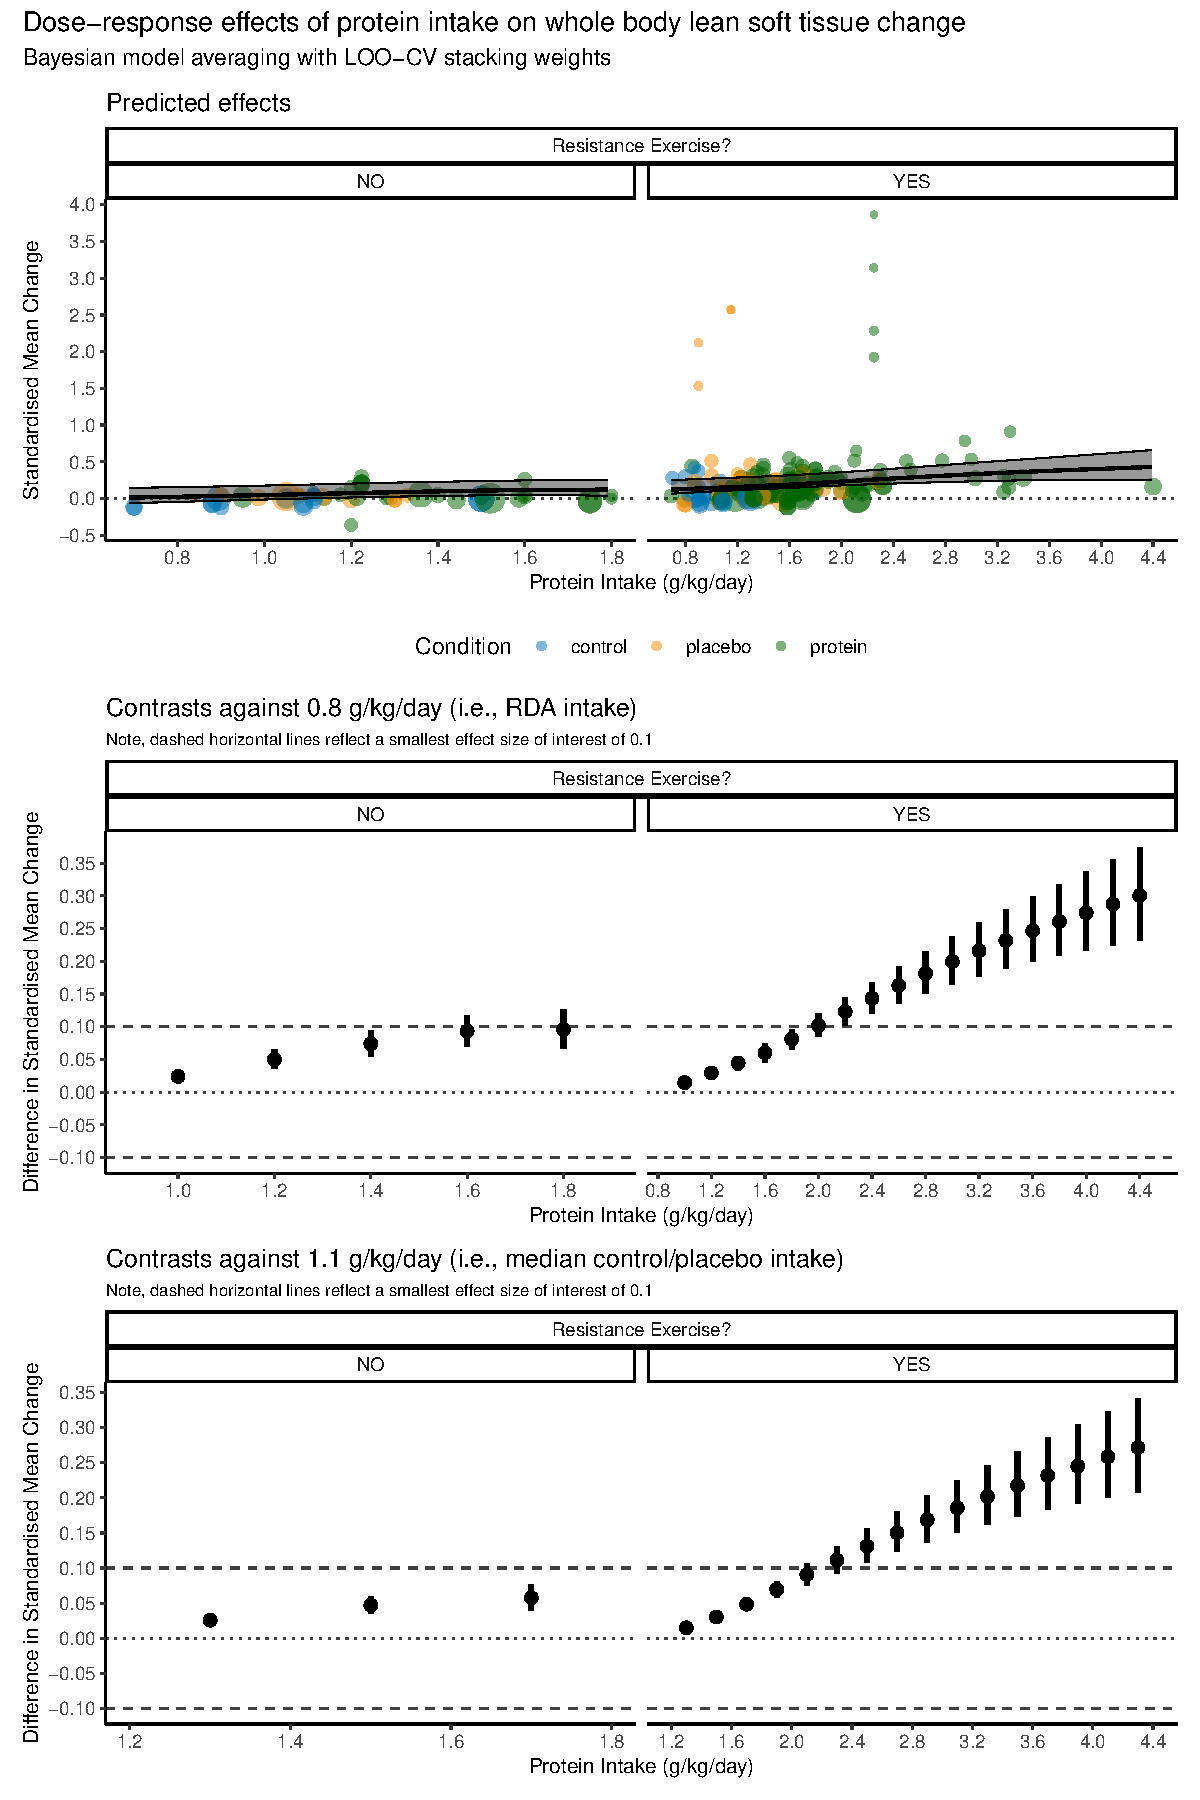
\includegraphics[keepaspectratio]{manuscript_files/figure-pdf/fig-whole-body-1.pdf}}

}

\caption{\label{fig-whole-body}Meta-analytic scatter plot of posterior
predictions for standardised mean change for whole body lean soft tissue
across protein intakes (top),contrasts of protein intakes against 0.8
g/kg/day (i.e., RDA intake) contrasts of protein intakes against 1.1
g/kg/day (i.e., median control/placebo intake) (bottom).}

\end{figure}%

\subsection{Direct muscle mass/size}\label{direct-muscle-masssize}

\begin{figure}

\centering{

\pandocbounded{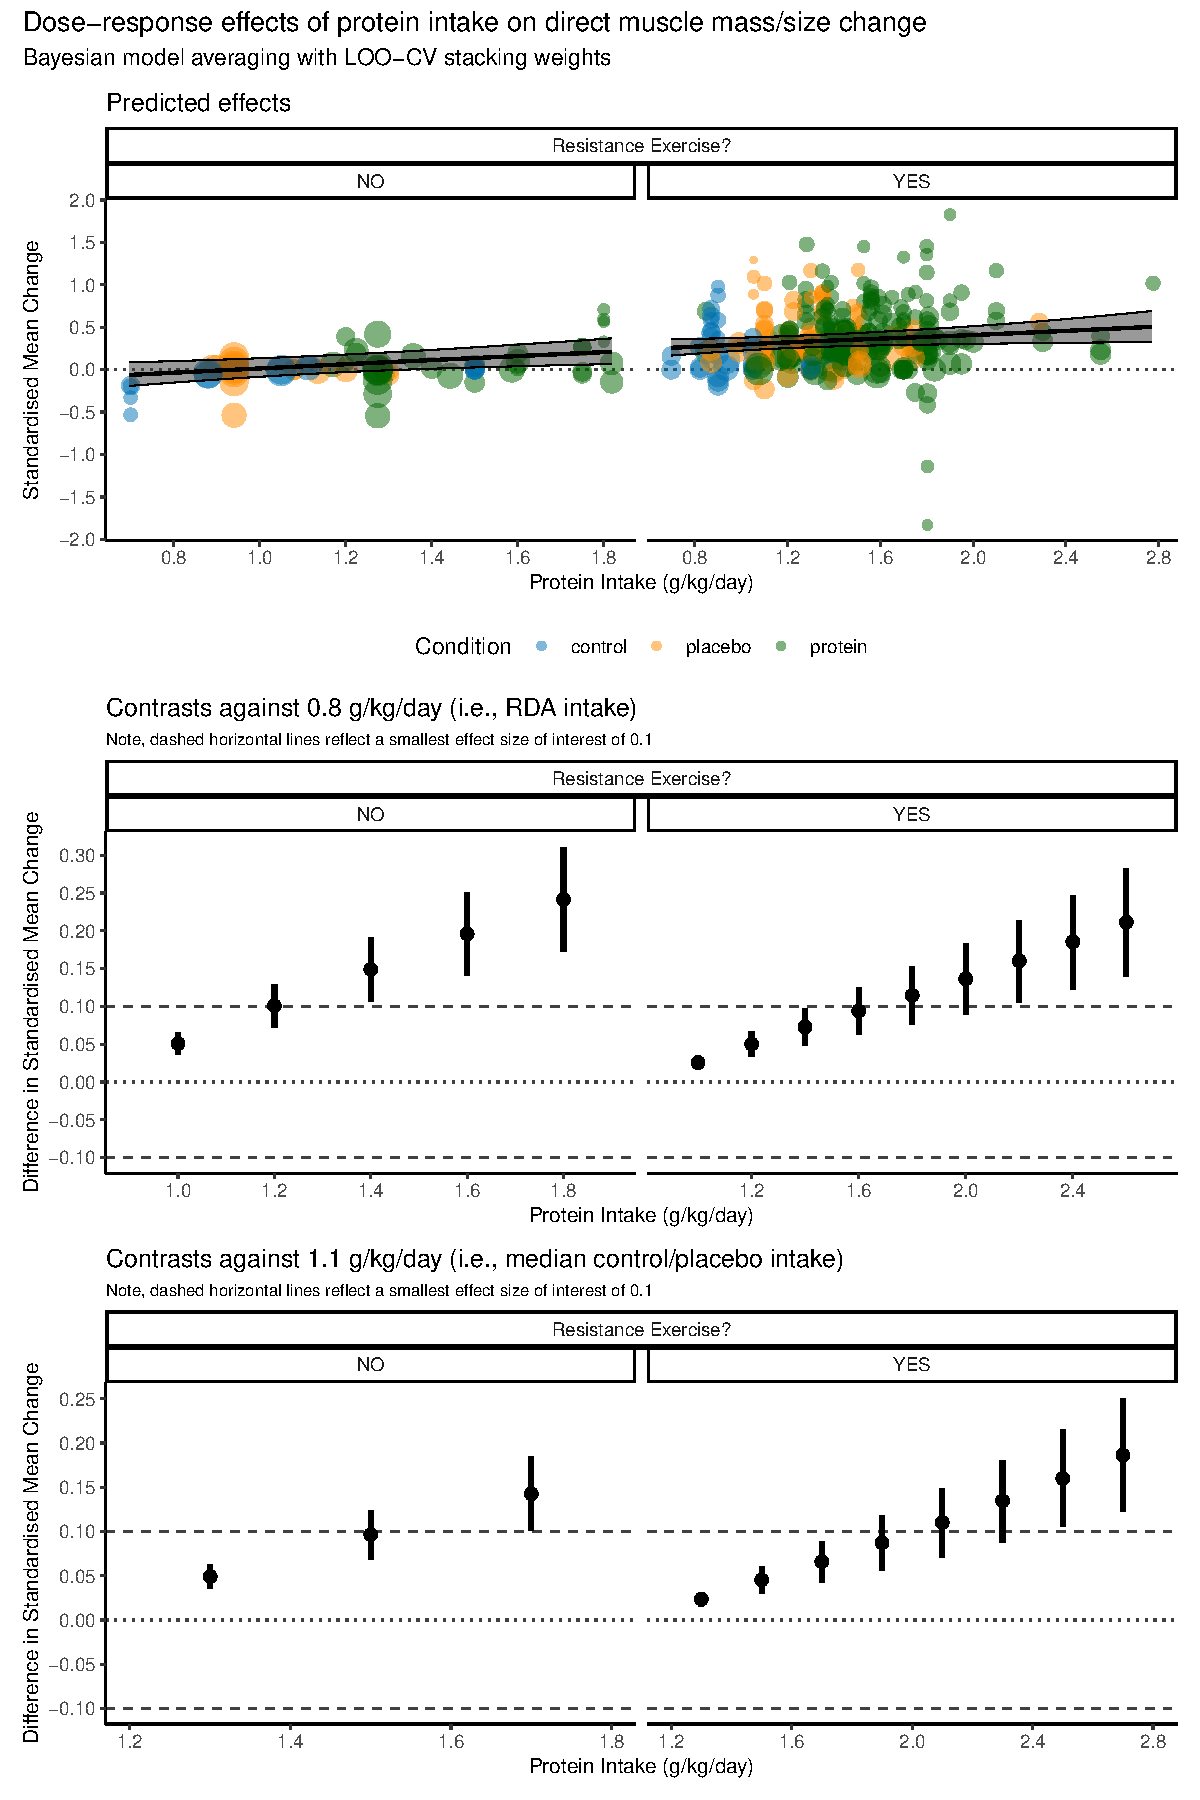
\includegraphics[keepaspectratio]{manuscript_files/figure-pdf/fig-hypertrophy-1.pdf}}

}

\caption{\label{fig-hypertrophy}Meta-analytic scatter plot of posterior
predictions for standardised mean change for direct muscle mass/size
across protein intakes (top),contrasts of protein intakes against 0.8
g/kg/day (i.e., RDA intake) contrasts of protein intakes against 1.1
g/kg/day (i.e., median control/placebo intake) (bottom).}

\end{figure}%

\subsection{Strength}\label{strength}

\begin{figure}

\centering{

\pandocbounded{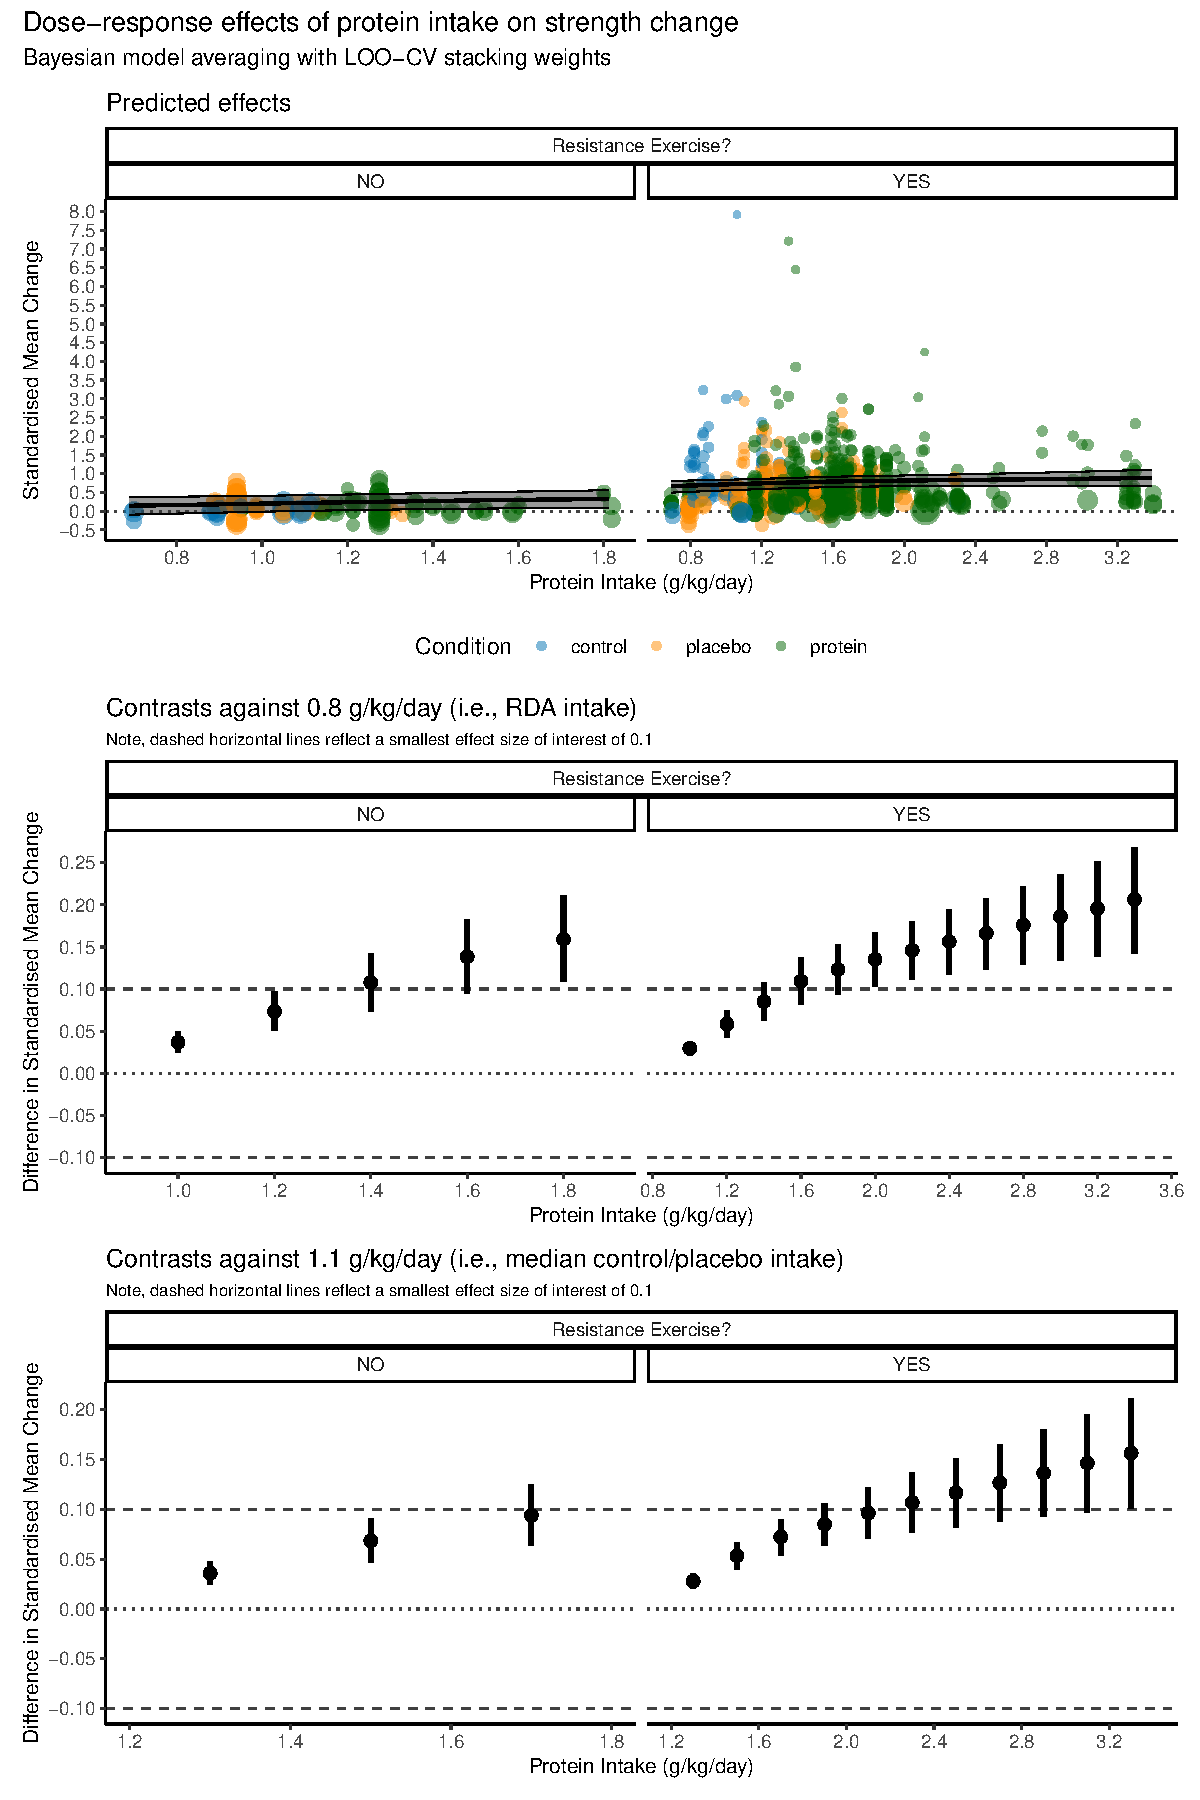
\includegraphics[keepaspectratio]{manuscript_files/figure-pdf/fig-strength-1.pdf}}

}

\caption{\label{fig-strength}Meta-analytic scatter plot of posterior
predictions for standardised mean change for strength across protein
intakes (top),contrasts of protein intakes against 0.8 g/kg/day (i.e.,
RDA intake) contrasts of protein intakes against 1.1 g/kg/day (i.e.,
median control/placebo intake) (bottom).}

\end{figure}%

\subsection{Function}\label{function}

\begin{figure}

\centering{

\pandocbounded{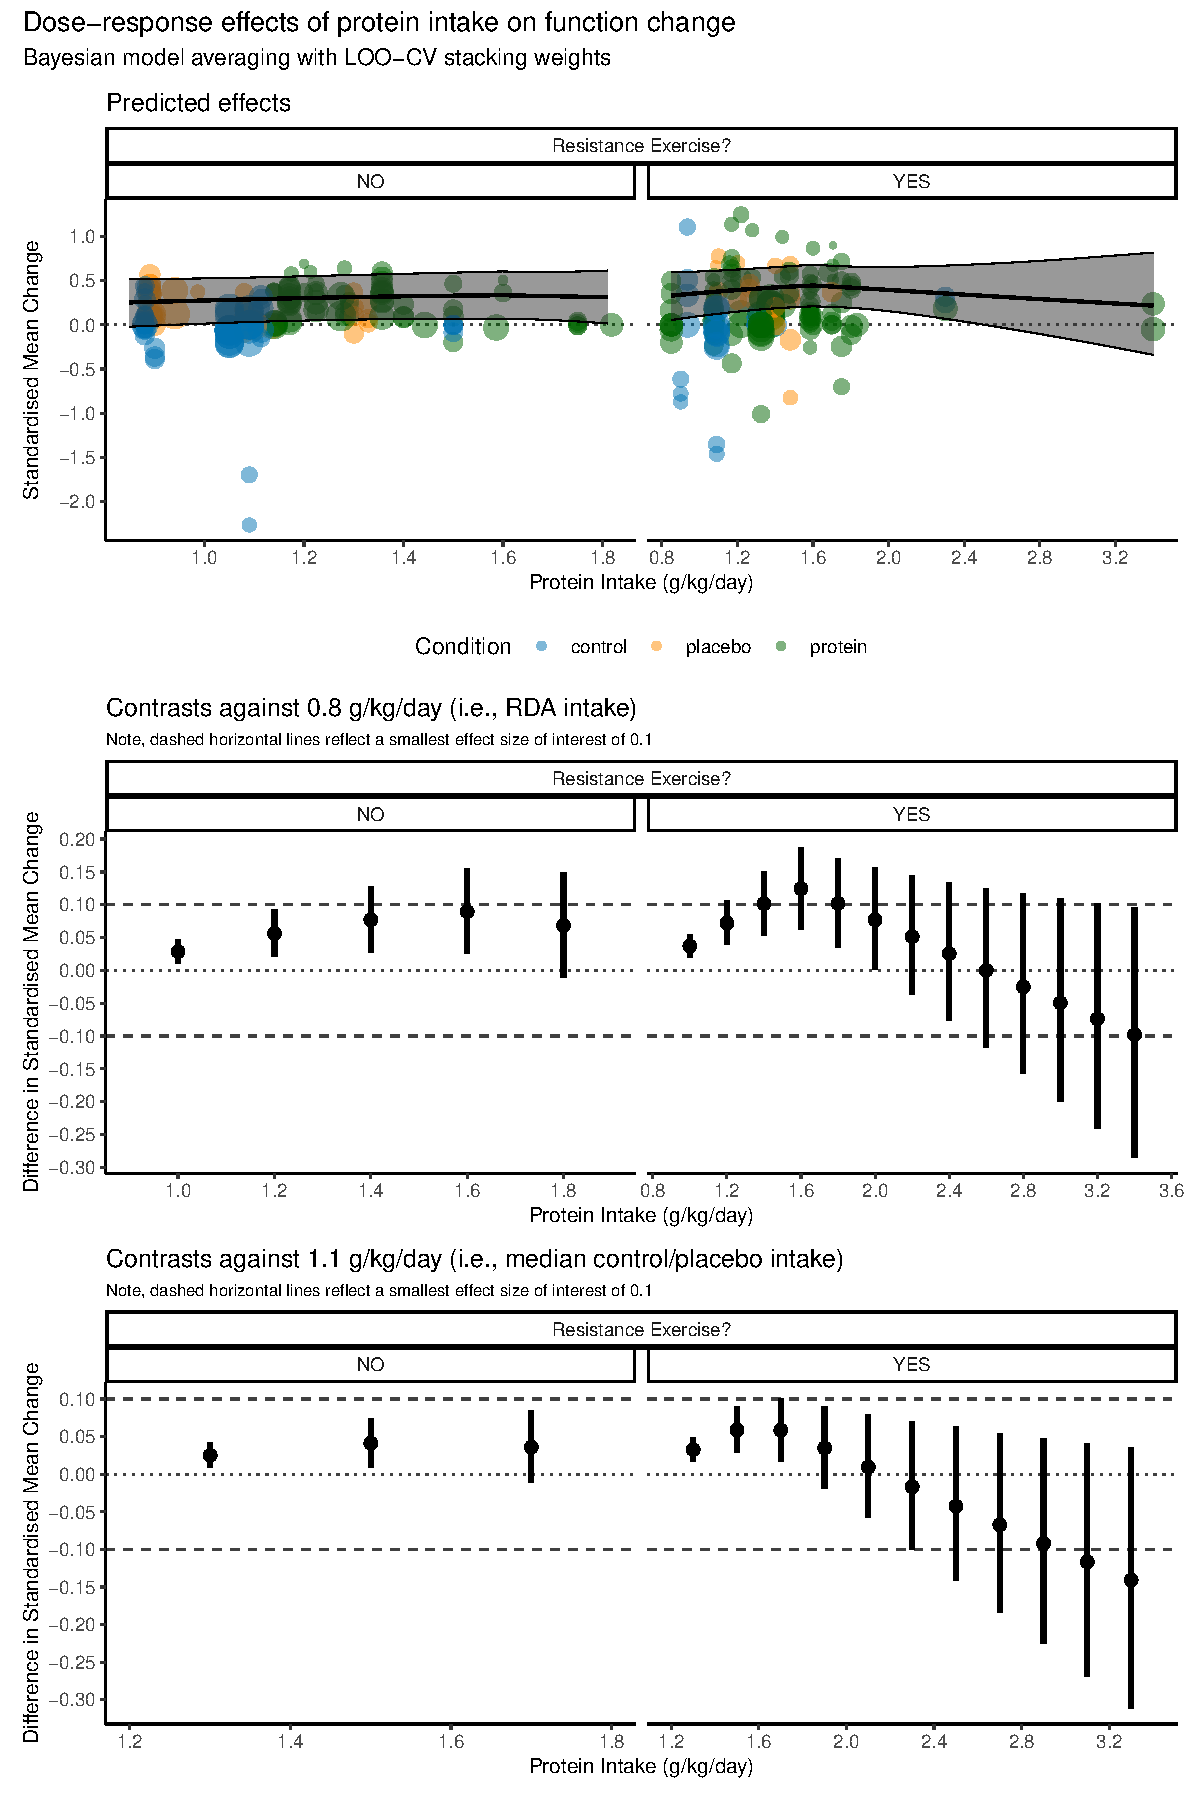
\includegraphics[keepaspectratio]{manuscript_files/figure-pdf/fig-function-1.pdf}}

}

\caption{\label{fig-function}Meta-analytic scatter plot of posterior
predictions for standardised mean change for function across protein
intakes (top),contrasts of protein intakes against 0.8 g/kg/day (i.e.,
RDA intake) contrasts of protein intakes against 1.1 g/kg/day (i.e.,
median control/placebo intake) (bottom).}

\end{figure}%

\begin{table}

\caption{\label{tbl-contrasts-rda}Percentage of posterior distribution
within the region of pratical equivalence (ROPE) and probability of
meaningful positive effects for contrasts of protein intakes against 0.8
g/kg/day (i.e., RDA intake).}

\centering{

\centering\centering
\begin{tabular}[t]{l|c|c|c|c|c|c|c|c}
\hline
\multicolumn{1}{c|}{ } & \multicolumn{2}{c|}{Whole body lean soft tissue} & \multicolumn{2}{c|}{Direct muscle mass/size} & \multicolumn{2}{c|}{Strength} & \multicolumn{2}{c}{Function} \\
\cline{2-3} \cline{4-5} \cline{6-7} \cline{8-9}
Contrast & Percentage within ROPE & Probability of meaningful positive effect & Percentage within ROPE & Probability of meaningful positive effect & Percentage within ROPE & Probability of meaningful positive effect & Percentage within ROPE & Probability of meaningful positive effect\\
\hline
\multicolumn{9}{l}{\textbf{Resistance Training = YES}}\\
\hline
\hspace{1em}1.0 versus 0.8 g/kg/day & 100.0\% & 0.0\% & 100.0\% & 0.0\% & 100.0\% & 0.0\% & 100.0\% & \vphantom{1} 0.0\%\\
\hline
\hspace{1em}1.2 versus 0.8 g/kg/day & 100.0\% & 0.0\% & 100.0\% & 0.0\% & 100.0\% & 0.0\% & 94.2\% & 5.8\%\\
\hline
\hspace{1em}1.4 versus 0.8 g/kg/day & 100.0\% & 0.0\% & 98.7\% & 1.3\% & 89.6\% & 10.4\% & 47.3\% & 52.7\%\\
\hline
\hspace{1em}1.6 versus 0.8 g/kg/day & 100.0\% & 0.0\% & 64.6\% & 35.4\% & 26.0\% & 74.0\% & 21.6\% & 78.4\%\\
\hline
\hspace{1em}1.8 versus 0.8 g/kg/day & 99.3\% & 0.7\% & 23.1\% & 76.9\% & 6.4\% & 93.6\% & 47.6\% & 52.4\%\\
\hline
\hspace{1em}2.0 versus 0.8 g/kg/day & 40.7\% & 59.2\% & 6.1\% & 93.9\% & 1.5\% & 98.5\% & 71.4\% & 28.6\%\\
\hline
\hspace{1em}2.2 versus 0.8 g/kg/day & 1.4\% & 98.6\% & 1.4\% & 98.6\% & 0.5\% & 99.5\% & 84.8\% & 15.2\%\\
\hline
\hspace{1em}2.4 versus 0.8 g/kg/day & 0.0\% & 100.0\% & 0.4\% & 99.6\% & 0.2\% & 99.8\% & 90.4\% & 8.7\%\\
\hline
\hspace{1em}2.6 versus 0.8 g/kg/day & 0.0\% & 100.0\% & 0.1\% & 99.9\% & 0.2\% & 99.8\% & 89.6\% & 5.6\%\\
\hline
\hspace{1em}2.8 versus 0.8 g/kg/day & 0.0\% & 100.0\% &  &  & 0.1\% & 99.9\% & 82.4\% & 4.0\%\\
\hline
\hspace{1em}3.0 versus 0.8 g/kg/day & 0.0\% & 100.0\% &  &  & 0.0\% & 100.0\% & 71.0\% & 3.1\%\\
\hline
\hspace{1em}3.2 versus 0.8 g/kg/day & 0.0\% & 100.0\% &  &  & 0.0\% & 100.0\% & 58.8\% & 2.7\%\\
\hline
\hspace{1em}3.4 versus 0.8 g/kg/day & 0.0\% & 100.0\% &  &  & 0.0\% & 100.0\% & 48.5\% & 2.3\%\\
\hline
\hspace{1em}3.6 versus 0.8 g/kg/day & 0.0\% & 100.0\% &  &  &  &  &  & \\
\hline
\hspace{1em}3.8 versus 0.8 g/kg/day & 0.0\% & 100.0\% &  &  &  &  &  & \\
\hline
\hspace{1em}4.0 versus 0.8 g/kg/day & 0.0\% & 100.0\% &  &  &  &  &  & \\
\hline
\hspace{1em}4.2 versus 0.8 g/kg/day & 0.0\% & 100.0\% &  &  &  &  &  & \\
\hline
\hspace{1em}4.4 versus 0.8 g/kg/day & 0.0\% & 100.0\% &  &  &  &  &  & \\
\hline
\multicolumn{9}{l}{\textbf{Resistance Training = NO}}\\
\hline
\hspace{1em}1.0 versus 0.8 g/kg/day & 100.0\% & 0.0\% & 100.0\% & 0.0\% & 100.0\% & 0.0\% & 100.0\% & 0.0\%\\
\hline
\hspace{1em}1.2 versus 0.8 g/kg/day & 100.0\% & 0.0\% & 48.3\% & 51.7\% & 98.4\% & 1.6\% & 99.1\% & 0.9\%\\
\hline
\hspace{1em}1.4 versus 0.8 g/kg/day & 99.4\% & 0.6\% & 1.1\% & 98.9\% & 32.8\% & 67.2\% & 81.0\% & 19.0\%\\
\hline
\hspace{1em}1.6 versus 0.8 g/kg/day & 70.3\% & 29.7\% & 0.0\% & 100.0\% & 4.1\% & 95.9\% & 62.4\% & 37.6\%\\
\hline
\multicolumn{9}{l}{\rule{0pt}{1em}\textit{Note: }}\\
\multicolumn{9}{l}{\rule{0pt}{1em}Note, the ROPE is the range determined by the smallest effect size of interest i.e., [-0.1, 0.1] and as such a meaningful positive effect is one which exceeds the upper limit i.e., >0.1)}\\
\end{tabular}

}

\end{table}%

\begin{table}

\caption{\label{tbl-contrasts-median}Percentage of posterior
distribution within the region of pratical equivalence (ROPE) and
probability of meaningful positive effects for contrasts of protein
intakes against 1.1 g/kg/day (i.e., median control/placebo intake).}

\centering{

\centering\centering
\begin{tabular}[t]{l|c|c|c|c|c|c|c|c}
\hline
\multicolumn{1}{c|}{ } & \multicolumn{2}{c|}{Whole body lean soft tissue} & \multicolumn{2}{c|}{Direct muscle mass/size} & \multicolumn{2}{c|}{Strength} & \multicolumn{2}{c}{Function} \\
\cline{2-3} \cline{4-5} \cline{6-7} \cline{8-9}
Contrast & Percentage within ROPE & Probability of meaningful positive effect & Percentage within ROPE & Probability of meaningful positive effect & Percentage within ROPE & Probability of meaningful positive effect & Percentage within ROPE & Probability of meaningful positive effect\\
\hline
\multicolumn{9}{l}{\textbf{Resistance Training = YES}}\\
\hline
\hspace{1em}1.3 versus 1.1 g/kg/day & 100.0\% & 0.0\% & 100.0\% & 0.0\% & 100.0\% & 0.0\% & 100.0\% & \vphantom{1} 0.0\%\\
\hline
\hspace{1em}1.5 versus 1.1 g/kg/day & 100.0\% & 0.0\% & 100.0\% & 0.0\% & 100.0\% & 0.0\% & 99.5\% & 0.5\%\\
\hline
\hspace{1em}1.7 versus 1.1 g/kg/day & 100.0\% & 0.0\% & 99.8\% & 0.2\% & 99.9\% & 0.1\% & 97.2\% & 2.8\%\\
\hline
\hspace{1em}1.9 versus 1.1 g/kg/day & 100.0\% & 0.0\% & 78.8\% & 21.2\% & 91.5\% & 8.5\% & 98.8\% & 1.2\%\\
\hline
\hspace{1em}2.1 versus 1.1 g/kg/day & 88.2\% & 11.8\% & 31.0\% & 69.0\% & 61.5\% & 38.5\% & 99.2\% & 0.7\%\\
\hline
\hspace{1em}2.3 versus 1.1 g/kg/day & 13.3\% & 86.7\% & 7.6\% & 92.4\% & 33.0\% & 67.0\% & 96.9\% & 0.6\%\\
\hline
\hspace{1em}2.5 versus 1.1 g/kg/day & 0.5\% & 99.5\% & 1.5\% & 98.5\% & 16.9\% & 83.1\% & 86.5\% & 0.5\%\\
\hline
\hspace{1em}2.7 versus 1.1 g/kg/day & 0.0\% & 100.0\% & 0.4\% & 99.6\% & 8.9\% & 91.1\% & 70.0\% & 0.4\%\\
\hline
\hspace{1em}2.9 versus 1.1 g/kg/day & 0.0\% & 100.0\% &  &  & 5.0\% & 95.0\% & 54.0\% & 0.4\%\\
\hline
\hspace{1em}3.1 versus 1.1 g/kg/day & 0.0\% & 100.0\% &  &  & 3.3\% & 96.7\% & 41.2\% & 0.4\%\\
\hline
\hspace{1em}3.3 versus 1.1 g/kg/day & 0.0\% & 100.0\% &  &  & 2.4\% & 97.6\% & 31.4\% & 0.4\%\\
\hline
\hspace{1em}3.5 versus 1.1 g/kg/day & 0.0\% & 100.0\% &  &  &  &  &  & \\
\hline
\hspace{1em}3.7 versus 1.1 g/kg/day & 0.0\% & 100.0\% &  &  &  &  &  & \\
\hline
\hspace{1em}3.9 versus 1.1 g/kg/day & 0.0\% & 100.0\% &  &  &  &  &  & \\
\hline
\hspace{1em}4.1 versus 1.1 g/kg/day & 0.0\% & 100.0\% &  &  &  &  &  & \\
\hline
\hspace{1em}4.3 versus 1.1 g/kg/day & 0.0\% & 100.0\% &  &  &  &  &  & \\
\hline
\multicolumn{9}{l}{\textbf{Resistance Training = NO}}\\
\hline
\hspace{1em}1.3 versus 1.1 g/kg/day & 100.0\% & 0.0\% & 100.0\% & 0.0\% & 100.0\% & 0.0\% & 100.0\% & 0.0\%\\
\hline
\hspace{1em}1.5 versus 1.1 g/kg/day & 100.0\% & 0.0\% & 59.9\% & 40.1\% & 99.7\% & 0.3\% & 100.0\% & 0.0\%\\
\hline
\hspace{1em}1.7 versus 1.1 g/kg/day & 100.0\% & 0.0\% & 2.3\% & 97.7\% & 65.0\% & 35.0\% & 99.5\% & 0.5\%\\
\hline
\multicolumn{9}{l}{\rule{0pt}{1em}\textit{Note: }}\\
\multicolumn{9}{l}{\rule{0pt}{1em}Note, the ROPE is the range determined by the smallest effect size of interest i.e., [-0.1, 0.1] and as such a meaningful positive effect is one which exceeds the upper limit i.e., >0.1)}\\
\end{tabular}

}

\end{table}%

\section{Discussion}\label{discussion}

\section{Conclusion}\label{conclusion}

Intakes up to \textasciitilde3 g/kg/day do not meaningfully improve
outcomes compared to 0.8 g/kg/day. Above this uncertainty in estimates
renders difficulty in determining whether effects are meaningful or not
with x-y\% probability of positive meaningful effects and x-y\%
probability of practically equivalent effects.

\protect\phantomsection\label{refs}
\begin{CSLReferences}{1}{0}
\bibitem[\citeproctext]{ref-beckerSynthesizingStandardizedMeanchange1988}
Becker, B. J. (1988). Synthesizing standardized mean-change measures.
\emph{British Journal of Mathematical and Statistical Psychology},
\emph{41}(2), 257--278.
\url{https://doi.org/10.1111/j.2044-8317.1988.tb00901.x}

\bibitem[\citeproctext]{ref-benitoSystematicReviewMetaAnalysis2020}
Benito, P. J., Cupeiro, R., Ramos-Campo, D. J., Alcaraz, P. E., \&
Rubio-Arias, J. Á. (2020). A {Systematic Review} with {Meta-Analysis} of
the {Effect} of {Resistance Training} on {Whole-Body Muscle Growth} in
{Healthy Adult Males}. \emph{International Journal of Environmental
Research and Public Health}, \emph{17}(4), 1285.
\url{https://doi.org/10.3390/ijerph17041285}

\bibitem[\citeproctext]{ref-bucknerDoseresponseRelationshipResistance2023a}
Buckner, S. L., Moreno, E. N., \& Baxter, H. T. (2023). The
dose-response relationship between resistance training volume and muscle
hypertrophy: {There} are still doubts. \emph{Journal of Trainology},
\emph{12}(2), 29--36. \url{https://doi.org/10.17338/trainology.12.2_29}

\bibitem[\citeproctext]{ref-heymsfieldAreLeanBody2024}
Heymsfield, S. B., Brown, J., Ramirez, S., Prado, C. M., Tinsley, G. M.,
\& Gonzalez, M. C. (2024). Are {Lean Body Mass} and {Fat-Free Mass} the
{Same} or {Different Body Components}? {A Critical Perspective}.
\emph{Advances in Nutrition}, \emph{15}(12), 100335.
\url{https://doi.org/10.1016/j.advnut.2024.100335}

\bibitem[\citeproctext]{ref-hinneConceptualIntroductionBayesian2020}
{Hinne, M., Gronau, Q. F., van den Bergh, D., \& Wagenmakers, E.-J.}
(2020). A {Conceptual Introduction} to {Bayesian Model Averaging}.
\emph{Advances in Methods and Practices in Psychological Science},
\emph{3}(2), 200--215. \url{https://doi.org/10.1177/2515245919898657}

\bibitem[\citeproctext]{ref-kirkMachineBasedResistanceTraining2024}
Kirk, A., Steele, J., \& Fisher, J. P. (2024). Machine-{Based Resistance
Training Improves Functional Capacity} in {Older Adults}: {A Systematic
Review} and {Meta-Analysis}. \emph{Journal of Functional Morphology and
Kinesiology}, \emph{9}(4), 239.
\url{https://doi.org/10.3390/jfmk9040239}

\bibitem[\citeproctext]{ref-kruschkeBayesianNewStatistics2018}
Kruschke, J. K., \& Liddell, T. M. (2018). The {Bayesian New
Statistics}: {Hypothesis} testing, estimation, meta-analysis, and power
analysis from a {Bayesian} perspective {[}Journal Article{]}.
\emph{Psychonomic Bulletin \& Review}, \emph{25}, 178--206.

\bibitem[\citeproctext]{ref-morrisEstimatingEffectSizes2008}
Morris, S. B. (2008). Estimating {Effect Sizes From
Pretest-Posttest-Control Group Designs}. \emph{Organizational Research
Methods}, \emph{11}(2), 364--386.
\url{https://doi.org/10.1177/1094428106291059}

\bibitem[\citeproctext]{ref-mortonSystematicReviewMetaanalysis2018}
Morton, R. W., Murphy, K. T., McKellar, S. R., Schoenfeld, B. J.,
Henselmans, M., Helms, E., Aragon, A. A., Devries, M. C., Banfield, L.,
Krieger, J. W., \& Phillips, S. M. (2018). A systematic review,
meta-analysis and meta-regression of the effect of protein
supplementation on resistance training-induced gains in muscle mass and
strength in healthy adults. \emph{British Journal of Sports Medicine},
\emph{52}(6), 376--384.
\url{https://doi.org/10.1136/bjsports-2017-097608}

\bibitem[\citeproctext]{ref-nunesSystematicReviewMetaanalysis2022}
Nunes, E. A., Colenso-Semple, L., McKellar, S. R., Yau, T., Ali, M. U.,
Fitzpatrick-Lewis, D., Sherifali, D., Gaudichon, C., Tomé, D., Atherton,
P. J., Robles, M. C., Naranjo-Modad, S., Braun, M., Landi, F., \&
Phillips, S. M. (2022). Systematic review and meta-analysis of protein
intake to support muscle mass and function in healthy adults.
\emph{Journal of Cachexia, Sarcopenia and Muscle}, \emph{13}(2),
795--810. \url{https://doi.org/10.1002/jcsm.12922}

\bibitem[\citeproctext]{ref-ouzzaniRayyanaWebMobile2016}
Ouzzani, M., Hammady, H., Fedorowicz, Z., \& Elmagarmid, A. (2016).
Rayyan-a web and mobile app for systematic reviews. \emph{Systematic
Reviews}, \emph{5}(1), 210.
\url{https://doi.org/10.1186/s13643-016-0384-4}

\bibitem[\citeproctext]{ref-pagePRISMA2020Statement2021}
Page, M. J., McKenzie, J. E., Bossuyt, P. M., Boutron, I., Hoffmann, T.
C., Mulrow, C. D., Shamseer, L., Tetzlaff, J. M., Akl, E. A., Brennan,
S. E., Chou, R., Glanville, J., Grimshaw, J. M., Hróbjartsson, A., Lalu,
M. M., Li, T., Loder, E. W., Mayo-Wilson, E., McDonald, S., \ldots{}
Moher, D. (2021). The {PRISMA} 2020 statement: An updated guideline for
reporting systematic reviews. \emph{BMJ}, \emph{372}, n71.
\url{https://doi.org/10.1136/bmj.n71}

\bibitem[\citeproctext]{ref-steeleMetaanalysisVariationSport2023}
Steele, J., Fisher, J. P., Smith, D., Schoenfeld, B. J., Yang, Y., \&
Nakagawa, S. (2023). Meta-analysis of variation in sport and exercise
science: {Examples} of application within resistance training research.
\emph{Journal of Sports Sciences}, \emph{41}(17), 1617--1634.
\url{https://doi.org/10.1080/02640414.2023.2286748}

\bibitem[\citeproctext]{ref-sterneRoB2Revised2019}
Sterne, J. A. C., Savović, J., Page, M. J., Elbers, R. G., Blencowe, N.
S., Boutron, I., Cates, C. J., Cheng, H.-Y., Corbett, M. S., Eldridge,
S. M., Emberson, J. R., Hernán, M. A., Hopewell, S., Hróbjartsson, A.,
Junqueira, D. R., Jüni, P., Kirkham, J. J., Lasserson, T., Li, T.,
\ldots{} Higgins, J. P. T. (2019). {RoB} 2: A revised tool for assessing
risk of bias in randomised trials. \emph{BMJ}, \emph{366}, l4898.
\url{https://doi.org/10.1136/bmj.l4898}

\bibitem[\citeproctext]{ref-tagawaSynergisticEffectIncreased2022}
Tagawa, R., Watanabe, D., Ito, K., Otsuyama, T., Nakayama, K., Sanbongi,
C., \& Miyachi, M. (2022). Synergistic {Effect} of {Increased Total
Protein Intake} and {Strength Training} on {Muscle Strength}: {A
Dose-Response Meta-analysis} of {Randomized Controlled Trials}.
\emph{Sports Medicine - Open}, \emph{8}(1), 110.
\url{https://doi.org/10.1186/s40798-022-00508-w}

\bibitem[\citeproctext]{ref-tagawaDoseResponseRelationship2021}
Tagawa, R., Watanabe, D., Ito, K., Ueda, K., Nakayama, K., Sanbongi, C.,
\& Miyachi, M. (2021). Dose--response relationship between protein
intake and muscle mass increase: A systematic review and meta-analysis
of randomized controlled trials. \emph{Nutrition Reviews}, \emph{79}(1),
66--75. \url{https://doi.org/10.1093/nutrit/nuaa104}

\bibitem[\citeproctext]{ref-vehtariPracticalBayesianModel2017}
Vehtari, A., Gelman, A., \& Gabry, J. (2017). Practical {Bayesian} model
evaluation using leave-one-out cross-validation and {WAIC}.
\emph{Statistics and Computing}, \emph{27}(5), 1413--1432.
\url{https://doi.org/10.1007/s11222-016-9696-4}

\bibitem[\citeproctext]{ref-yaoUsingStackingAverage2018}
Yao, Y., Vehtari, A., Simpson, D., \& Gelman, A. (2018). Using
{Stacking} to {Average Bayesian Predictive Distributions} (with
{Discussion}). \emph{Bayesian Analysis}, \emph{13}(3), 917--1007.
\url{https://doi.org/10.1214/17-BA1091}

\end{CSLReferences}




\end{document}
